% ==============================================================================
% Diagrama de Sequência Compacto para Dissertação de Mestrado (LaTeX / TikZ)
% Obra: RDL-N1: Governança por Regras e Políticas e Mitigação de Conflitos no Near-RT RIC
% Autor: George Alexandro Ferreira Barbosa | PPGCOMP / UFPA
% Fluxo implementado em src/ (revisado em 2026-11-08). Sem valores medidos:
% os tempos são parâmetros de configuração; a troca E2 real ainda não foi exercitada.
% ==============================================================================

\documentclass[tikz,border=5mm]{standalone}
\usepackage[utf8]{inputenc}
\usepackage[T1]{fontenc}
\usepackage{amsmath,amssymb}
\usepackage{tikz}
\usetikzlibrary{arrows.meta,positioning,calc}

\begin{document}
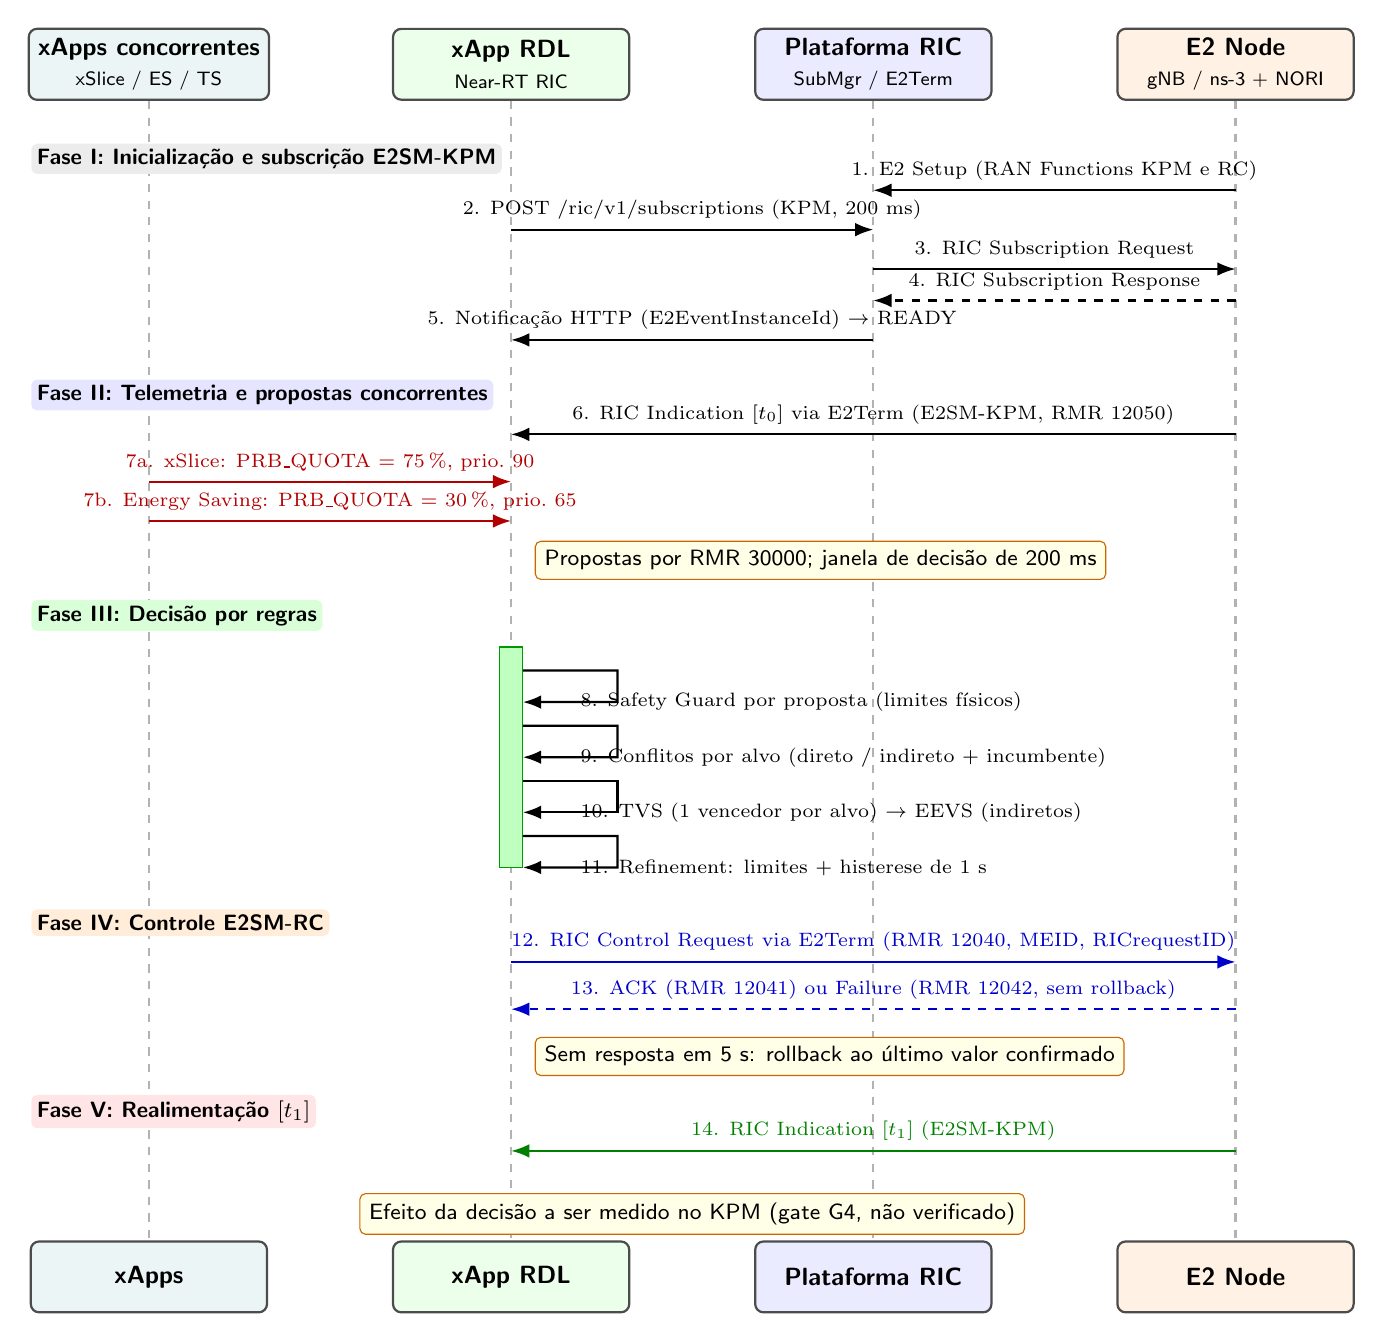
\begin{tikzpicture}[
    font=\sffamily\small,
    entity/.style={draw=black!70, fill=white, rounded corners=3pt, thick, minimum width=3.0cm, minimum height=0.9cm, align=center},
    lifeline/.style={draw=black!30, dashed, thick},
    msg/.style={-{Latex}, thick},
    note/.style={draw=orange!80!black, fill=yellow!10, rounded corners=2pt, font=\sffamily\footnotesize, align=left},
    phase/.style={anchor=west, font=\sffamily\bfseries\footnotesize, inner sep=2pt, rounded corners=2pt}
]

    % Participantes
    \def\xXAPP{0}
    \def\xRDL{4.6}
    \def\xRIC{9.2}
    \def\xRAN{13.8}
    \def\yTop{0}
    \def\yBottom{-15.4}

    \node[entity, fill=teal!8] (xappTop) at (\xXAPP, \yTop) {\textbf{xApps concorrentes}\\\scriptsize xSlice / ES / TS};
    \node[entity, fill=green!8] (rdlTop) at (\xRDL, \yTop) {\textbf{xApp RDL}\\\scriptsize Near-RT RIC};
    \node[entity, fill=blue!8] (ricTop) at (\xRIC, \yTop) {\textbf{Plataforma RIC}\\\scriptsize SubMgr / E2Term};
    \node[entity, fill=orange!10] (ranTop) at (\xRAN, \yTop) {\textbf{E2 Node}\\\scriptsize gNB / ns-3 + NORI};

    \node[entity, fill=teal!8] (xappBot) at (\xXAPP, \yBottom) {\textbf{xApps}};
    \node[entity, fill=green!8] (rdlBot) at (\xRDL, \yBottom) {\textbf{xApp RDL}};
    \node[entity, fill=blue!8] (ricBot) at (\xRIC, \yBottom) {\textbf{Plataforma RIC}};
    \node[entity, fill=orange!10] (ranBot) at (\xRAN, \yBottom) {\textbf{E2 Node}};

    \draw[lifeline] (xappTop.south) -- (xappBot.north);
    \draw[lifeline] (rdlTop.south) -- (rdlBot.north);
    \draw[lifeline] (ricTop.south) -- (ricBot.north);
    \draw[lifeline] (ranTop.south) -- (ranBot.north);

    % Fase I
    \node[phase, fill=gray!15] at (-1.5, -1.2) {Fase I: Inicialização e subscrição E2SM-KPM};
    \draw[msg] (\xRAN, -1.6) -- node[above, font=\scriptsize] {1. E2 Setup (RAN Functions KPM e RC)} (\xRIC, -1.6);
    \draw[msg] (\xRDL, -2.1) -- node[above, font=\scriptsize] {2. POST /ric/v1/subscriptions (KPM, 200 ms)} (\xRIC, -2.1);
    \draw[msg] (\xRIC, -2.6) -- node[above, font=\scriptsize] {3. RIC Subscription Request} (\xRAN, -2.6);
    \draw[msg, dashed] (\xRAN, -3.0) -- node[above, font=\scriptsize] {4. RIC Subscription Response} (\xRIC, -3.0);
    \draw[msg] (\xRIC, -3.5) -- node[above, font=\scriptsize] {5. Notificação HTTP (E2EventInstanceId) $\rightarrow$ READY} (\xRDL, -3.5);

    % Fase II
    \node[phase, fill=blue!10] at (-1.5, -4.2) {Fase II: Telemetria e propostas concorrentes};
    \draw[msg] (\xRAN, -4.7) -- node[above, font=\scriptsize] {6. RIC Indication $[t_0]$ via E2Term (E2SM-KPM, RMR 12050)} (\xRDL, -4.7);
    \draw[msg, color=red!70!black] (\xXAPP, -5.3) -- node[above, font=\scriptsize] {7a. xSlice: PRB\_QUOTA = 75\,\%, prio.\ 90} (\xRDL, -5.3);
    \draw[msg, color=red!70!black] (\xXAPP, -5.8) -- node[above, font=\scriptsize] {7b. Energy Saving: PRB\_QUOTA = 30\,\%, prio.\ 65} (\xRDL, -5.8);
    \node[note, anchor=west] at (\xRDL + 0.3, -6.3) {Propostas por RMR 30000; janela de decisão de 200 ms};

    % Fase III
    \node[phase, fill=green!15] at (-1.5, -7.0) {Fase III: Decisão por regras};
    \draw[fill=green!25, draw=green!60!black] (\xRDL - 0.15, -7.4) rectangle (\xRDL + 0.15, -10.2);
    \draw[msg] (\xRDL + 0.15, -7.7) -- ++(1.2,0) -- ++(0,-0.4) -- node[right, font=\scriptsize] {8. Safety Guard por proposta (limites físicos)} (\xRDL + 0.15, -8.1);
    \draw[msg] (\xRDL + 0.15, -8.4) -- ++(1.2,0) -- ++(0,-0.4) -- node[right, font=\scriptsize] {9. Conflitos por alvo (direto / indireto + incumbente)} (\xRDL + 0.15, -8.8);
    \draw[msg] (\xRDL + 0.15, -9.1) -- ++(1.2,0) -- ++(0,-0.4) -- node[right, font=\scriptsize] {10. TVS (1 vencedor por alvo) $\rightarrow$ EEVS (indiretos)} (\xRDL + 0.15, -9.5);
    \draw[msg] (\xRDL + 0.15, -9.8) -- ++(1.2,0) -- ++(0,-0.4) -- node[right, font=\scriptsize] {11. Refinement: limites + histerese de 1 s} (\xRDL + 0.15, -10.2);

    % Fase IV
    \node[phase, fill=orange!15] at (-1.5, -10.9) {Fase IV: Controle E2SM-RC};
    \draw[msg, color=blue!80!black] (\xRDL, -11.4) -- node[above, font=\scriptsize] {12. RIC Control Request via E2Term (RMR 12040, MEID, RICrequestID)} (\xRAN, -11.4);
    \draw[msg, dashed, color=blue!80!black] (\xRAN, -12.0) -- node[above, font=\scriptsize] {13. ACK (RMR 12041) ou Failure (RMR 12042, sem rollback)} (\xRDL, -12.0);
    \node[note, anchor=west] at (\xRDL + 0.3, -12.6) {Sem resposta em 5 s: rollback ao último valor confirmado};

    % Fase V
    \node[phase, fill=red!10] at (-1.5, -13.3) {Fase V: Realimentação $[t_1]$};
    \draw[msg, color=green!50!black] (\xRAN, -13.8) -- node[above, font=\scriptsize] {14. RIC Indication $[t_1]$ (E2SM-KPM)} (\xRDL, -13.8);
    \node[note, anchor=center] at (6.9, -14.6) {Efeito da decisão a ser medido no KPM (gate G4, não verificado)};

\end{tikzpicture}
\end{document}
